%tikz
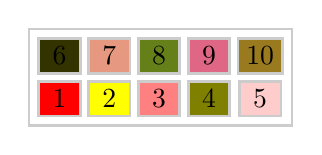
\begin{tikzpicture}[every node/.style={draw,scale=1pt,minimum width=15pt,inner sep=3pt,line width=1pt,draw=black!20}]
\matrix[row sep=2pt,column sep=2pt]
{\node[fill=-blue!20]{6};&
\node[fill=red!80!green!50]{7};&
\node[fill=-blue!80!red!50]{8};&
\node[fill=red!80!blue!60]{9};&
\node[fill=-blue!80!green!60]{10};\\
\node[fill=red]{1};&
\node[fill=-blue]{2};&
\node[fill=red!50]{3};&
\node[fill=-blue!50]{4};&
\node[fill=red!20]{5};\\
};
\end{tikzpicture}
